\section{ТАСКЛЕТЫ}

\begin{lstlisting}[caption=Текст программы]
#include <linux/module.h>
#include <linux/kernel.h>
#include <linux/init.h>
#include <linux/interrupt.h>
#include <linux/time.h>

#define HANDLEDIRQ 1

MODULE_AUTHOR("Alexander Stepanov");
MODULE_LICENSE("GPL");

static int irq = HANDLEDIRQ;
static int irq_call_count = 0;
static int dev_id;
char tasklet_data[] = "tasklet_function was called";

void tasklet_function(unsigned long data);

DECLARE_TASKLET(tasklet, tasklet_function, (unsigned long)&tasklet_data);

void tasklet_function(unsigned long data)
{
    struct timeval t;
    struct tm brocken;
    do_gettimeofday(&t);
    time_to_tm(t.tv_sec, 0, &brocken);

    printk(KERN_INFO
        "[tasklet_module] Tasklet: { state: %ld, count: %d, data: %s },"
        "current_time: %d:%d:%d:%ld\n",
        tasklet.state, atomic_read(&tasklet.count), (char *)tasklet.data,
        brocken.tm_hour + 3, brocken.tm_min, brocken.tm_sec, t.tv_usec);
}

static irqreturn_t interrupt_handler(int irq, void *dev_id)
{
    if (irq == HANDLEDIRQ)
    {
        irq_call_count++;
        printk(KERN_INFO
            "[tasklet_module] irq call count = %d\n", irq_call_count);
        tasklet_schedule(&tasklet);
        return IRQ_HANDLED;
    }
    else
    {
        return IRQ_NONE;
    }
}

static int __init tasklet_module_init(void)
{
    int ret = request_irq(
        irq, interrupt_handler, IRQF_SHARED,
        "tasklet_interrupt_handler", &dev_id
    );

    if (ret)
    {
        printk(KERN_ERR "[tasklet_module] error while handle irq\n");
        return -1;
    }

    printk(KERN_INFO "[tasklet_module] success load\n");
    return 0;
}

static void __exit tasklet_module_exit(void)
{
    tasklet_kill(&tasklet);
    free_irq(irq, &dev_id);
    printk(KERN_INFO "[tasklet_module] unload module\n");
}

module_init(tasklet_module_init);
module_exit(tasklet_module_exit);
\end{lstlisting}

\begin{figure}[H]
    \centering
    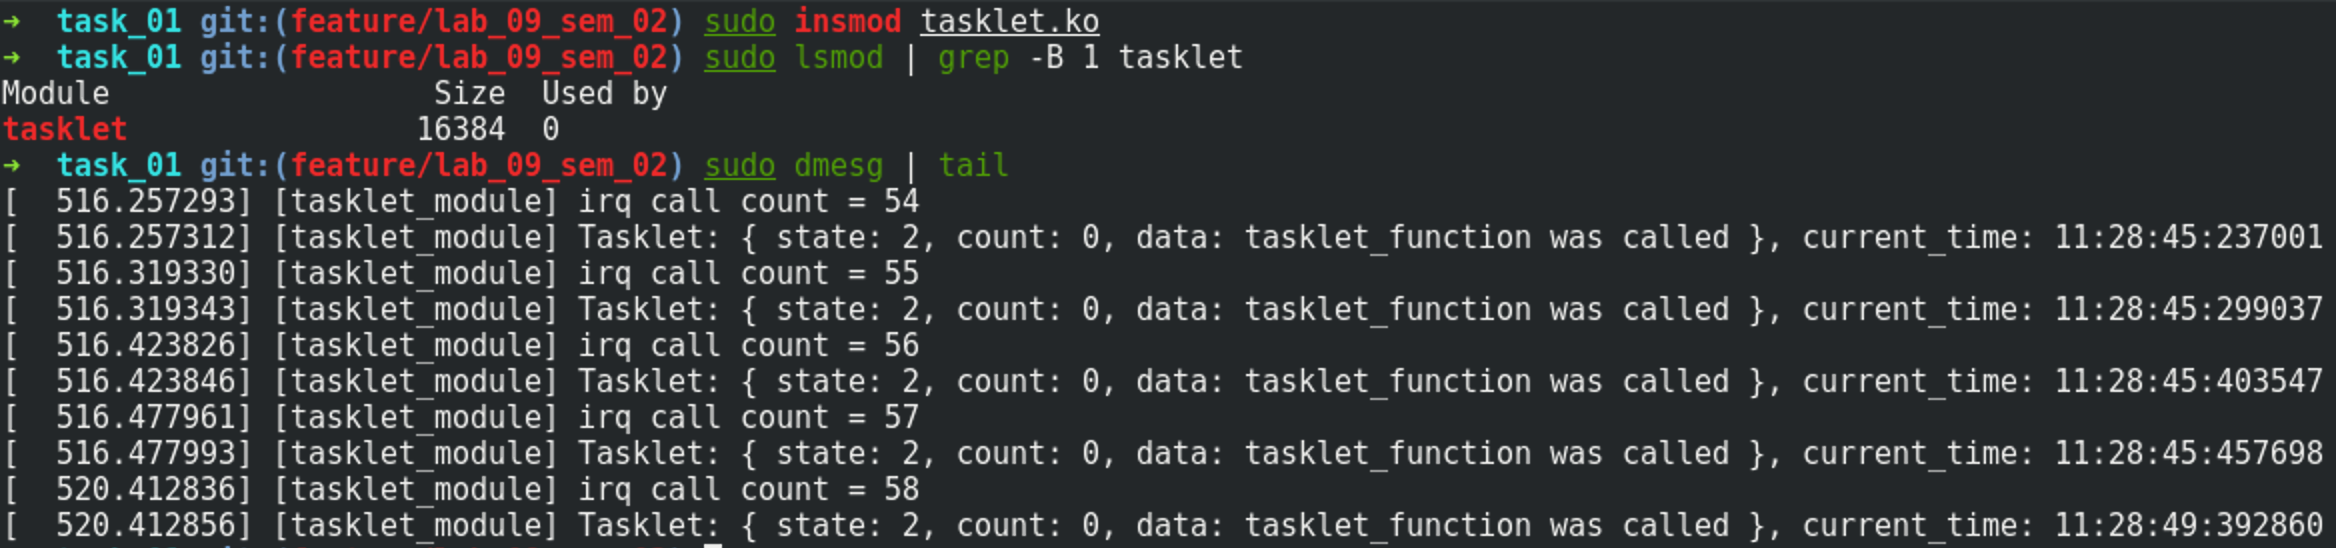
\includegraphics[scale=0.45]{img/part_01/insmod.png}
    \caption{Загрузка модуля}
\end{figure}

\begin{figure}[H]
    \centering
    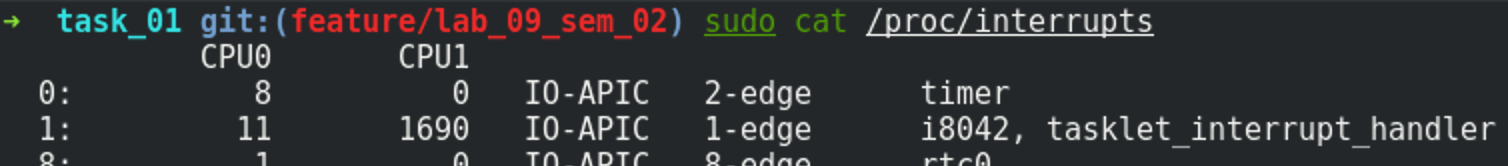
\includegraphics[scale=0.7]{img/part_01/interrupt.png}
    \caption{Прерывания}
\end{figure}

\begin{figure}[H]
    \centering
    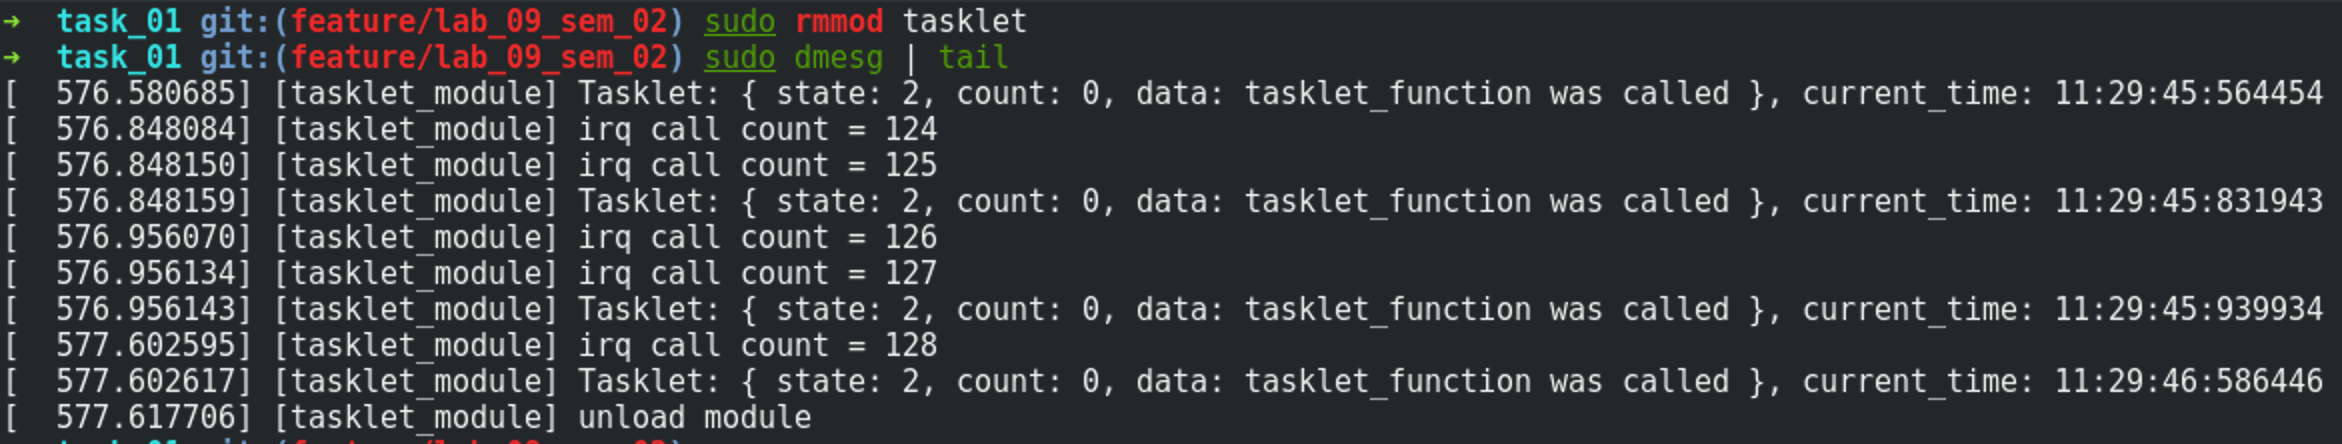
\includegraphics[scale=0.45]{img/part_01/rmmod.png}
    \caption{Выгрузка модуля}
\end{figure}

\section{ОЧЕРЕДИ РАБОТ}

\begin{lstlisting}[caption=Текст программы]
#include <linux/module.h>
#include <linux/kernel.h>
#include <linux/init.h>
#include <linux/interrupt.h>
#include <linux/workqueue.h>
#include <linux/time.h>

#define HANDLEDIRQ 1

MODULE_AUTHOR("Alexander Stepanov");
MODULE_LICENSE("GPL");

static int irq = HANDLEDIRQ;
static int irq_call_count = 0;
static int dev_id;
static struct workqueue_struct *workq = NULL;

void work_function(struct work_struct *work)
{
    struct timeval t;
    struct tm brocken;
    do_gettimeofday(&t);
    time_to_tm(t.tv_sec, 0, &brocken);

    printk(KERN_INFO
        "[workqueue_module] work: { data: %ld },"
        "current_time: %d:%d:%d:%ld\n",
        atomic_long_read(&work->data),
        brocken.tm_hour + 3, brocken.tm_min, brocken.tm_sec, t.tv_usec);
}

DECLARE_WORK(work, work_function);

static irqreturn_t interrupt_handler(int irq, void *dev_id)
{
    if (irq == HANDLEDIRQ)
    {
        irq_call_count++;
        queue_work(workq, &work);
        printk(KERN_INFO
            "[workqueue_module] irq call count = %d\n", irq_call_count);
        return IRQ_HANDLED;
    }
    else
    {
        return IRQ_NONE;
    }

}

static int __init workqueue_module_init(void)
{
    int ret = request_irq(
        irq, interrupt_handler, IRQF_SHARED,
        "workqueue_interrupt_handler", &dev_id
    );

    if (ret)
    {
        printk(KERN_ERR "[workqueue_module] error while handle irq\n");
        return -1;
    }

    workq = create_workqueue("workqueue");

    if (workq == NULL)
    {
        printk(KERN_ERR "[workqueue_module] error while create workqueue\n");
        return -1;
    }

    printk(KERN_INFO "[workqueue_module] success load\n");
    return 0;
}

static void __exit workqueue_module_exit(void)
{
    flush_workqueue(workq);
    destroy_workqueue(workq);
    free_irq(irq, &dev_id);
    printk(KERN_INFO "[workqueue_module] unload module\n");
}

module_init(workqueue_module_init);
module_exit(workqueue_module_exit);
\end{lstlisting}

\begin{figure}[H]
    \centering
    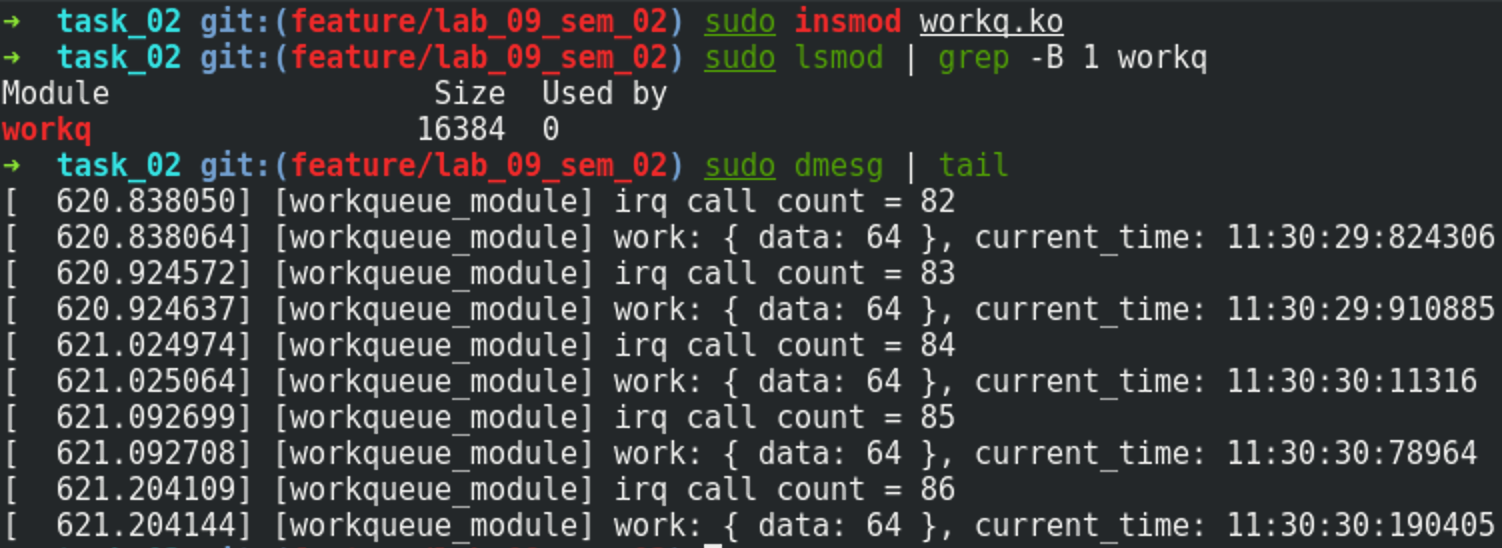
\includegraphics[scale=0.7]{img/part_02/insmod.png}
    \caption{Загрузка модуля}
\end{figure}

\begin{figure}[H]
    \centering
    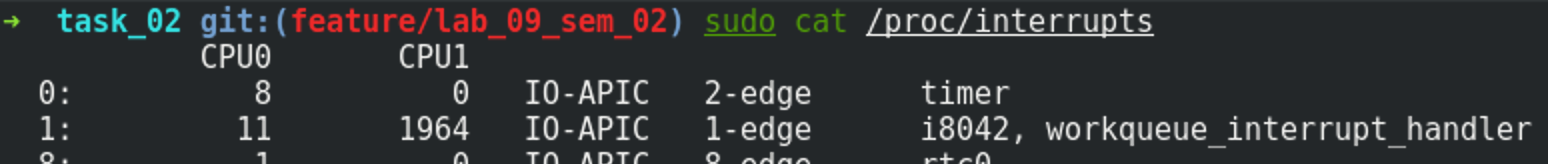
\includegraphics[scale=0.7]{img/part_02/interrupt.png}
    \caption{Прерывания}
\end{figure}

\begin{figure}[H]
    \centering
    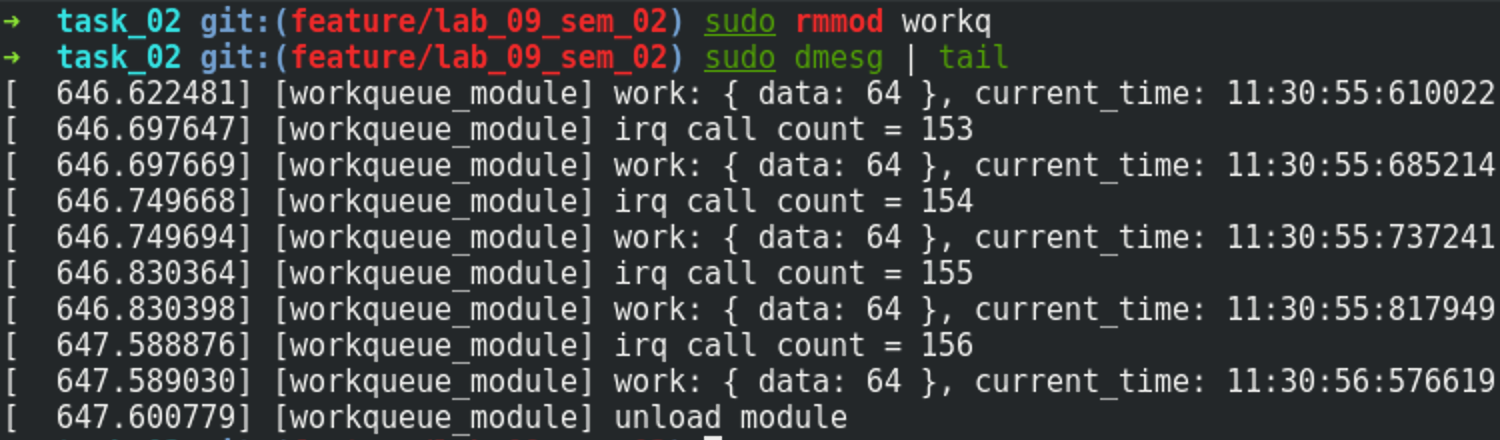
\includegraphics[scale=0.7]{img/part_02/rmmod.png}
    \caption{Выгрузка модуля}
\end{figure}
